\chapter{\IFRU{BPF: установка прерывания на исполнение функции}{BPF: set breakpoint on function execution}}

\IFRU{Опция BPF, в каком-то смысле, похожа на работу утилиты}{BPF option, in a way, it is a kind of} strace\footnote{\url{http://en.wikipedia.org/wiki/Strace}}.

\IFRU{Главные отличия от strace:}{Significant differences with strace are:}

\begin{itemize}
\item tracer \IFRU{работает только в win32/win64.}{is win32/win64 only.}
\item \IFRU{Прерыванием может быть любоая функция а не только системные вызовы.}{Breakpoints not just system calls, but any function.}
\item \IFRU{Только 4 прерывания из-за ограничений архитектуры x86.}{Only 4 breakpoints, because of x86 architecture limitation.}
\end{itemize}

\IFRU{BPF с адресом но без дополнительных опций будет только показывать момент вызова функции и то что она возвращает.}{BPF option with address without additional options will only track the moment when function was called and what it returns.}

\forexample{}

\begin{lstlisting}
tracer.exe -l:bzip2.exe bpf=kernel32.dll!WriteFile
\end{lstlisting}

\begin{lstlisting}
1188 (0) KERNEL32.dll!WriteFile () (called from 0x610AC912 (cygwin1.dll!sigemptyset+0x1022))
1188 (0) KERNEL32.dll!WriteFile -> 1
\end{lstlisting}

\IFRU{Замечание: tracer не знает о том что функция может иметь тип \IT{void} (т.е., не возвращает ничего). Таким образом, tracer выводит просто то что находится в регистре \TT{EAX}/\TT{RAX} на момент выхода из функции.}{Note: tracer doesn't know some function is void type, e.g., it doesn't return any value. So it just takes the value at \TT{EAX}/\TT{RAX} register.}

\IFRU{Опции}{Options}:

\TT{ARGS:<number>}: \IFRU{определить количество агрументов для перехватываемой функции}{define arguments number for the function we would like to intercept}.

\forexample{}

\begin{lstlisting}
tracer.exe -l:bzip2.exe -c:--help bpf=kernel32.dll!WriteFile,args:5
\end{lstlisting}

\begin{lstlisting}
09D0 (0) KERNEL32.dll!WriteFile (0x0000001B, "   If no file names are given, bzip2 compresses or decompresses", 0x0000003F, "?", 0)
09D0 (0) KERNEL32.dll!WriteFile -> 1
09D0 (0) KERNEL32.dll!WriteFile (0x0000001B, "   from standard input to standard output.  You can combinesses", 0x0000003B, ";", 0)
09D0 (0) KERNEL32.dll!WriteFile -> 1
09D0 (0) KERNEL32.dll!WriteFile (0x0000001B, "   short flags, so `-v -4' means the same as -v4 or -4v, &amp;c.ses", 0x0000003C, "<", 0)
09D0 (0) KERNEL32.dll!WriteFile -> 1
\end{lstlisting}

\IFRU{То что мы видим это попытку вывести 5 агрументов функции при каждом вызове функции WriteFile().}{What we see here is an attempt to read 5 arguments at each WriteFile function call.}
\IFRU{Если аргумент является указателем в пределах памяти процесса и то на что он указывает может быть интерпретировано как ASCII-строка, она будет выведена.}{If some of these arguments are pointers to some area within process memory, and the data at the pointer can be interpreted as ASCII string, it will be printed instead.}
\IFRU{Это очень удобно для перехвата строковых функций таких как strcmp(), strlen(), strtok(), atoi(), итд.}{This is useful when intercepting string functions like strcmp(), strlen(), strtok(), atoi(), and so on.}

\IFRU{Ошибится в количестве аргументов не страшно (кроме случая использования опции \TT{skip\_stdcall}, смотрите ниже). Если указанное количество аргументов больше чем на самом деле, возможно, значения из локальных переменных вызывающей функции будут выведены. Или какой-нибудь случайный мусор. Если заданное количество аргументов меньше чем на самом деле, только часть аргументов будет выведена.}{It is not a problem to make mistake on arguments number (except using \TT{skip\_stdcall} option, see below). If defined arguments number greater than real, captured local variables of caller function probably will be printed. Or any other useless junk. If defined arguments number is less than real, then only part of arguments will be visible.}

\TT{RT:<number>}: \IFRU{подставить другое возвращаемое значение в момент выхода из функции, на лету.}{replace the returning value of any function by something else, on fly.}

\begin{lstlisting}
tracer.exe -l:filename.exe bpf=function,args:1,rt:0x12345678
\end{lstlisting}

tracer \IFRU{запишет это значение в регистр \TT{EAX}/\TT{RAX} в момент выхода из функции.}{will put this value to \TT{EAX}/\TT{RAX} right at the moment when function exited.}

\TT{SKIP}: \IFRU{пропустить выполнение функции. Эта опция может использоваться вместе с опцией \TT{RT}.}{bypass a function. This can be used with \TT{RT} option too.}

\begin{lstlisting}
tracer.exe -l:filename.exe bpf=function,args:1,rt:0x12345678,skip
\end{lstlisting}

\IFRU{Это означает что в момент начала выполнения функции, управление сразу будет передано на выход и возвращаемое значение будет установлено в 0x12345678.}{This means that the function just gets bypassed and its return value is fixed at 0x12345678.}

\IFRU{Замечание: без префикса "0x", это значение будет интерпретироваться как десятичное число.}{Note: without "0x" prefix, this value would be interpreted as decimal number.}

\TT{SKIP\_STDCALL}: \IFRU{то же что и \TT{SKIP}, только для stdcall-функций.}{the same as <b>SKIP</b> option but rather used for stdcall functions.}

\IFRU{Разница между типами функций cdecl и stdcall в том что функция типа сdecl на выходе не выравнивает указатель стека (вызывающая функция должна сделать это). Функция типа stdcall выравнивает указатель стека. cdecl это наиболее используемый тип функций. Хотя, stdcall используется в MS Windows. Так что, если вы хотите пропустить выполнение какой-либо функции в KERNEL32.DLL или USER32.DLL, вы должны использовать \TT{skip\_stdcall}. Следовательно, в этом случае, tracer должен знать точное количество аргументов, а без этого процесс может упасть.}{The difference between cdecl and stdcall calling conventions is just that cdecl function doesn't align stack pointer at exit (caller should do this). stdcall function aligns stack pointer at exit. cdecl is the most used calling convention. However, stdcall is used in MS Windows. So, if you would like to skip a function in KERNEL32.DLL or USER32.DLL, you should use \TT{skip\_stdcall}. Consequently, in this case, gt must know the exact arguments number, without it the process may crash.}\footnote{\IFRU{Смотрите также}{See also}: X86 calling conventions\url{http://en.wikipedia.org/wiki/X86_calling_conventions}}

\IFRU{Если вы хотите подавить все вызовы функции WriteFile:}{If you'd like to suppress all WriteFile calls, do this:}

\begin{lstlisting}
tracer.exe -l:hello.exe bpf=kernel32.dll!WriteFile,args:5,skip_stdcall,rt:1
\end{lstlisting}

\IFRU{Не забывайте возвращать 1, для того чтобы вызываемая функция не заподозрила ничего!}{Don't forget to make it return 1, so the caller will not suspect anything!}
\IFRU{Количество аргументов функции WriteFile --- 5. Поменяйте это значение на что-то другое и процесс упадет.}{WriteFile arguments number is just 5. Change it to something different, and process crashes.}

\IFRU{Замечание: тип функции stdcall отсутствует в Windows x64, так что эта опция отсутствует в 64-битной версии tracer.}{Note: stdcall calling convention is absent in Windows x64, so this option is absent in win64-version of tracer.}

\TT{UNICODE}: \IFRU{трактовать строки в аргументах как юникодные (два байта на каждый символ). Это может быть полезно для перехвата win32-функций с суффиксом W, например, MessageBoxW.}{treat strings in arguments as unicode (widechar). This could be helpful if you intercept unicode win32 functions with W suffix, for example, MessageBoxW.}

\IFRU{К сожалению, tracer умеет автоматически выявлять только строки использующие первую половину таблицы ASCII, так что строки на других языках кроме тех что используют латиницу не будут выявлены автоматически.}{Unfortunately, gt can only automatically detect first half of ASCII table, so multilingual unicode strings will not be detected.}

\TT{DUMP\_ARGS:<size>}: \IFRU{дампить память по аргументам функции (если она чиается) с ограничением size.}{dump memory on argument (if readable) limited by max size.}

\IFRU{Если аргумент функции содержит указатель на читаемый блок памяти, он будет выведен.}{If argument contain pointer to valid memory block, it will be printed.}

\IFRU{На момент выхода из функции, если блок в памяти изменился, то разница будет выведена также.}{At the function exit, if memory block contents was changed, difference will be printed too.}

\forexample{}

\begin{lstlisting}
tracer64.exe -l:test_getlocaltime.exe bpf=.*!getlocaltime,args:1,dump_args:0x30
\end{lstlisting}

\begin{lstlisting}
TID=6660|(0) KERNEL32.dll!GetLocalTime (0x12ff00) (called from 0x14000100f (getlocaltime.exe!BASE+0x100f))
Dump of buffer at argument 1 (starting at 1)
000000000012FF00: 28 FF 12 00 00 00 00 00-00 00 00 00 00 00 00 00 "(..............."
000000000012FF10: 01 00 00 00 00 00 00 00-73 11 00 40 01 00 00 00 "........s..@...."
000000000012FF20: 00 00 00 00 00 00 00 00-00 00 00 00 00 00 00 00 "................"
TID=6660|(0) KERNEL32.dll!GetLocalTime -> 0x150
Dump difference of buffer at argument 1 (starting at 1)
0000000000000000: D9 07 0C    06    05   -05    10    24    50 01 "... . . . . $ P."
\end{lstlisting}

\IFRU{Таким образом мы можем увидеть как win32-функция GetLocalTime() заполняет структуру SYSTEMTIME.}{Now we can see how GetLocalTime win32 function fill SYSTEMTIME structure.}

\section{\IFRU{Опция TRACE}{TRACE option}}

\TT{TRACE}: \IFRU{трассировать функцию по одной инструкции и сохранять значения всех интересующих нас регистров. После исполнения, эта информация сохранится в файлы process.exe.idc, process.exe.txt, process.exe\_clear.idc. .idc-файлы являются скриптами для IDA, а к .txt файлу можно применять grep, awk, sed для поиска интересующих нас значений.}{trace each instruction in function and collect all interesting values from registers and memory. After execution, all that information is saved to process.exe.idc, process.exe.txt, process.exe\_clear.idc files. .idc-files are IDA scripts, .txt file is grepable by grep, awk and sed.}

\IFRU{Возьмем для примера функцию add\_member из статьи}{For example, let's take add\_member function from} \IT{Using Uninitialized Memory for Fun and Profit}\footnote{\url{http://research.swtch.com/2008/03/using-uninitialized-memory-for-fun-and.html}}\IFRU{}{article}:

\begin{lstlisting}
int dense[256];
int dense_next=0;
int sparse[256];

void add_member(int i)
{
	dense[dense_next]=i;
	sparse[i]=dense_next;
	dense_next++;

};

int main ()
{
	add_member(123);
	add_member(5);
	add_member(71);
	add_member(99);
}
\end{lstlisting}

\IFRU{Скомпилируем и запустим трассировку на функции add\_member (вначале узнайте адрес функции при помощи IDA):}{Let's compile it and run tracing on add\_member function (determine function address in IDA before):}

\begin{lstlisting}
tracer -l:trace_test4.exe bpf=0x00401000,trace:cc
\end{lstlisting}

\IFRU{Получим файл trace\_test4.exe.txt:}{We'll get trace\_test4.exe.txt file:}

\begin{lstlisting}
0x401000, e=       4
0x401001, e=       4
0x401003, e=       4, [0x403818]=0..3
0x401008, e=       4, [EBP+8]=5, 0x47('G'), 0x63('c'), 0x7b('{')
0x40100b, e=       4, ECX=5, 0x47('G'), 0x63('c'), 0x7b('{')
0x401012, e=       4, [EBP+8]=5, 0x47('G'), 0x63('c'), 0x7b('{')
0x401015, e=       4, [0x403818]=0..3
0x40101a, e=       4, EAX=0..3
0x401021, e=       4, [0x403818]=0..3
0x401027, e=       4, ECX=0..3
0x40102a, e=       4, ECX=1..4
0x401030, e=       4
0x401031, e=       4, EAX=0..3
\end{lstlisting}

\IFRU{Поле \IT{e} - это сколько раз была исполнена эта инструкция.}{\IT{e} field is how many times was executed this instruction.}

\IFRU{Загрузим trace\_test4.exe.idc в IDA и увидим:}{Let's execute trace\_test4.exe.idc script in IDA and we'll see:}

\begin{figure}[ht!]
\centering
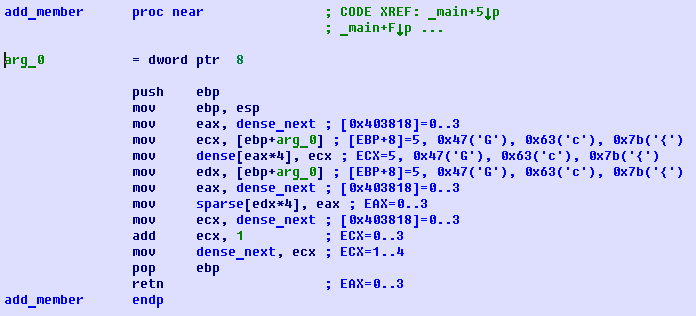
\includegraphics[scale=0.66]{trace_test4.png}
\caption{trace\_test4.png}
\end{figure}

\IFRU{Понимать работу функции во время исполнения, таким образом, становится намного проще.}{Now it is much simpler to understand how this function work during execution.}

\IFRU{Исполненные инструкции подсвечиваются голубым цветом. Неисполненные остаются белыми.}{Executed instructions are highlighed by blue color. Not-executed instructions are leaved white.}

\IFRU{Чтобы стереть все комментарии и подсветку, нужно исполнить скрипт trace\_test4.exe\_clear.idc}{If you need to clear all comments and highlight, execute trace\_test4.exe\_clear.idc script.}

\IFRU{Информация в IDA-скрипте может приводится в сокращенной форме из-за того что IDA имеет ограничение на длину комментария, например: \TT{EAX=[ 64 unique items. min=0xbca6eb7, max=0xffffffed ]}. В текстовом же файле сохраняется всё, поэтому иногда этот файл может оказаться в итоге очень большим.}{All collected information in IDA-script may be reduced to shorten form like \IT{EAX=[ 64 unique items. min=0xbca6eb7, max=0xffffffed ]} (because IDA has comment size limitation). On contrary, everything is saved to text file without shortening, that is why resulting text file may be sometimes pretty big.}

\IFRU{Недостаток опции TRACE в том что она работает медленно, хотя и функции в системных DLL пропускаются (системной считается та DLL которая находится внутри \%SystemRoot\%) Вторая проблема в том что пока что не очень корректно трассируются вещи вроде исключений, setjmp/longjmp и подобных непредвиденных изменений пути исполнения кода.}{One problem of TRACE feature that it is slow, however, functions from system DLLs are skipped (system DLL is that DLL residing in \%SystemRoot\%) Another problem is that things like exceptions, setjmp/longjmp and other unexpected codeflow alterations are not correctly handled so far.}



\section{\IFRU{Примеры}{Examples}}

\subsection{\IFRU{Простое использование}{Simple usage}}

\begin{lstlisting}
tracer.exe -l:bzip2.exe bpf=.*!fprintf,args:3
\end{lstlisting}

\begin{lstlisting}
TID=5128|(0) cygwin1.dll!fprintf (0x61103150, "%s: I won't write compressed data to a terminal.\n", "bzip2") (called from 0x401e03 (bzip2.exe!BASE+0x1e03))
TID=5128|(0) cygwin1.dll!fprintf -> 0x34
TID=5128|(0) cygwin1.dll!fprintf (0x61103150, "%s: For help, type: `%s --help'.\n", "bzip2") (called from 0x401c66 (bzip2.exe!BASE+0x1c66))
TID=5128|(0) cygwin1.dll!fprintf -> 0x27
\end{lstlisting}

\subsection{\IFRU{Перехват некоторых Windows-функций для работы с реестром}{Intercept some Windows registry access functions}}

\begin{lstlisting}
tracer.exe -l:someprocess.exe bpf=advapi32.dll!RegOpenKeyExA,args:5 bpf=advapi32.dll!RegQueryValueExA,args:6 bpf=advapi32.dll!RegSetValueExA,args:6
\end{lstlisting}

.. \IFRU{или измените суффиксы функция на W и добавьте опцию UNICODE}{or change function suffixes to W and add UNICODE option}:

\begin{lstlisting}
tracer64.exe -l:far.exe bpf=advapi32.dll!RegOpenKeyExW,args:5,unicode bpf=advapi32.dll!RegQueryValueExW,args:6,unicode bpf=advapi32.dll!RegSetValueExW,args:6,unicode
\end{lstlisting}

\subsection{\IFRU{Подавить шумный сигнал}{Suppress noisy beeping}}

\begin{lstlisting}
tracer.exe -l:beeper.exe bpf=kernel32.dll!Beep,args:2,skip_stdcall,rt:1
\end{lstlisting}

\subsection{\IFRU{Подавить диалоговое окно с сообщением}{Suppress Message Box}}

... \IFRU{и сделать так что вызываемая функция будет считать что пользователь каждый раз нажимает OK (константа IDOK равняется 1)}{by making it appear to a caller that the user presses OK every time (IDOK constant is 1)}:

\begin{lstlisting}
tracer.exe -l:filename.exe bpf=user32.dll!MessageBoxA,args:4,skip_stdcall,rt:1
\end{lstlisting}

... \IFRU{или CANCEL (константа IDCANCEL равняется 2)}{or CANCEL (IDCANCEL constant is 2)}:

\begin{lstlisting}
tracer.exe -l:filename.exe bpf=user32.dll!MessageBoxA,args:4,skip_stdcall,rt:2
\end{lstlisting}

\subsection{\IFRU{Перехват вызовов rand()}{Intercepting rand() call}}

\IFRU{Бывает весело перехватывать вызовы функции rand() в различных играх. Например, пасьянс Solitaire в Windows использует его для того чтобы сгенерировать случайный расклад. Мы можем установить возвращаемое значение rand() в ноль, и тогда Solitaire будет раздавать один и тот же расклад, всегда:}{Another fun is intercepting rand() function in various games. For example, Windows Solitaire card game use it to generate random deal. We can fix rand() return at zero, and Solitaire will do the same deal each time, forever:}

\IFRU{В}{In} Windows XP x86/x64:

\begin{lstlisting}
tracer.exe/tracer64.exe -l:c:\windows\system32\sol.exe bpf=.*!rand,rt:0
\end{lstlisting}

\IFRU{В}{In} Windows 7 x64:

\begin{lstlisting}
tracer64.exe -l:[full path to]\Solitaire.exe bpf=.*!rand,rt:0
\end{lstlisting}

\subsection{FreeCell}

\IFRU{Когда вы запускаете FreeCell в Windows (XP SP3) и нажимаете F2 (Новая игра), вы видите сообщение "Do you want to resign this game?" Мы можем подавить звуковой сигнал и сделать так что FreeCall будет думать что пользователь всегда нажимает YES:}{When you run Windows (XP SP3) FreeCell and press F2 (New game), you will get a message box "Do you want to resign this game?" We can suppress all that beeping and also make illusion to FreeCell user always press YES:}

\IFRU{Константа IDYES - 6. FreeCell использует функцию MessageBoxW - суффикс W означает уникодную версию функции MessageBox.}{IDYES constant is 6. FreeCell use MessageBoxW - W mean unicode version of MessageBox.}

\IFRU{В}{In} Windows XP SP3 x86:

\begin{lstlisting}
tracer.exe -l:c:\windows\system32\freecell.exe bpf=user32.dll!messagebeep,args:1,skip_stdcall bpf=user32.dll!messageboxw,args:4,unicode,skip_stdcall,rt:6
\end{lstlisting}

\begin{lstlisting}
TID=444|(0) USER32.dll!MessageBeep (0x20) (called from 0x1001f52 (freecell.exe!BASE+0x1f52))
We skip execution of this function
TID=444|(1) USER32.dll!MessageBoxW (0x80122, L"Do you want to resign this game?", L"FreeCell", 0x24) (called from 0x1001f5f (freecell.exe!BASE+0x1f5f))
We skip execution of this function
TID=444|We modify return value (EAX) of this function to 6
\end{lstlisting}

\IFRU{В}{In} Windows XP SP2 x64 Russian:

\begin{lstlisting}
tracer64.exe -l:c:\windows\system32\freecell.exe bpf=user32.dll!messagebeep,args:1,skip bpf=user32.dll!messageboxw,args:4,unicode,skip,rt:6
\end{lstlisting}

\begin{lstlisting}
TID=2028|(0) USER32.dll!MessageBeep (0x20) (called from 0x1000023f9 (freecell.exe!BASE+0x23f9))
We skip execution of this function
TID=2028|(1) USER32.dll!MessageBoxW (0x1f00f0, 0xbf80, 0xbf20, 0x24) (called from 0x100002416 (freecell.exe!BASE+0x2416))
We skip execution of this function
TID=2028|We modify return value (RAX) of this function to 6
\end{lstlisting}

\subsection{\IFRU{Проверка ивентов и запись в лог в Oracle RDBMS}{Oracle RDBMS Events checking and log writes}}

\IFRU{В}{In} Oracle 10.2.0.1 win64:

\begin{lstlisting}
tracer64.exe -a:oracle.exe bpf=oracle.exe!ksdpec,args:1 bpf=oracle.exe!ss_wrtf,args:3
\end{lstlisting}

( \IFRU{Смотрите также}{See also}: \url{http://blog.yurichev.com/node/14} )

\begin{lstlisting}
TID=3032|(0) oracle.exe!ksdpec (0x2743) (called from 0x9580a9 (oracle.exe!opiodr+0x105))
TID=3032|(0) oracle.exe!ksdpec -> 0xff
TID=3032|(1) oracle.exe!ss_wrtf (0x4a0, "*** 2009-12-04 06:19:01.005\n", 0x1b) (called from 0x45318d (oracle.exe!sdpri+0x22d))
TID=3032|(1) oracle.exe!ss_wrtf -> 1
TID=3032|(1) oracle.exe!ss_wrtf (0x4a0, "OPI CALL: type=107 argc= 3 cursor=  0 name=SES OPS (80)\n", 0x37) (called from 0x45318d (oracle.exe!sdpri+0x22d))
TID=3032|(1) oracle.exe!ss_wrtf -> 1
TID=3032|(0) oracle.exe!ksdpec (0x2743) (called from 0x9580a9 (oracle.exe!opiodr+0x105))
TID=3032|(0) oracle.exe!ksdpec -> 0xff
TID=3032|(1) oracle.exe!ss_wrtf (0x4a0, "OPI CALL: type=59 argc= 4 cursor=  0 name=VERSION2\n", 0x32) (called from 0x45318d (oracle.exe!sdpri+0x22d))
TID=3032|(1) oracle.exe!ss_wrtf -> 1
TID=3032|(0) oracle.exe!ksdpec (0x273e) (called from 0x4a00cc (oracle.exe!kslwte_tm+0x7a8))
TID=3032|(0) oracle.exe!ksdpec -> 0
TID=3032|(0) oracle.exe!ksdpec (0x273e) (called from 0x4a00cc (oracle.exe!kslwte_tm+0x7a8))
TID=3032|(0) oracle.exe!ksdpec -> 0
TID=3032|(0) oracle.exe!ksdpec (0x2743) (called from 0x9580a9 (oracle.exe!opiodr+0x105))
TID=3032|(0) oracle.exe!ksdpec -> 0xff
TID=3032|(1) oracle.exe!ss_wrtf (0x4a0, "OPI CALL: type=104 argc=12 cursor=  0 name=Transaction Commit/Rollback\n", 0x46) (called from 0x45318d (oracle.exe!sdpri+0x22d))
TID=3032|(1) oracle.exe!ss_wrtf -> 1
\end{lstlisting}

\subsection{\IFRU{Слежение за выделением памяти в}{Trace memory allocations in} Oracle 11.1.0.6.0 win32/win64}

\begin{lstlisting}
tracer.exe/tracer64.exe -a:oracle.exe bpf=.*!kghalf,args:6 bpf=.*!kghfrf,args:4
\end{lstlisting}

\begin{lstlisting}
TID=1600|(0) oracle.exe!kghalf (0x6d35af0, 0xb507ef8, 0x1000, 0, 0, "kzsrcrdi") (called from 0x1c7aa83 (oracle.exe!kzctxhugi+0x71))
TID=1600|(0) oracle.exe!kghalf -> 0xfa3ea58

TID=1600|(0) oracle.exe!kghalf (0x6d35af0, 0xb507ef8, 0x58, 1, 0x6d35530, "UPI heap") (called from 0x1e7f8b7 (oracle.exe!__PGOSF266_kwqmahal+0x5b))
TID=1600|(0) oracle.exe!kghalf -> 0xfa4d0d8

TID=1188|(0) oracle.exe!kghalf (0xda39540, 0xda39240, 0x88, 0, "ksirmdt array", 0xda39240) (called from 0x6afb5b (oracle.exe!ksz_nfy_ipga+0xf1))
TID=1188|(0) oracle.exe!kghalf -> 0x105d0b10

TID=1188|(0) oracle.exe!kghalf (0xda39540, 0xda39240, 0x48, 1, 0x1204e400, "local") (called from 0x3684a64 (oracle.exe!kjztcxini+0x58))
TID=1188|(0) oracle.exe!kghalf -> 0x105d0ab0
\end{lstlisting}

\subsection{\IFRU{Слежение за разбором SQL-выражений в}{SQL statements parsing in} Oracle RDBMS}

\IFRU{В}{In} Oracle 11.1.0.6.0 win32/win64:

\begin{lstlisting}
tracer.exe/tracer64.exe -a:oracle.exe bpf=oracle.exe!_?rpisplu,args:8 bpf=oracle.exe!_?kprbprs,args:7 bpf=oracle.exe!_?opiprs,args:6 bpf=oraclient11.dll!OCIStmtPrepare,args:6</i></p>
\end{lstlisting}

\IFRU{Замечание: регулярное выражение \IT{\_?function} покрывает оба имени: \TT{function} и \TT{\_function}.}{Note: regular expression \TT{\_?function} cover both \TT{function} and \TT{\_function}.}

\begin{lstlisting}
TID=1140|(2) oracle.exe!opiprs (0x13f029d0, "select 1 from obj$ where name='DBA_QUEUE_SCHEDULES'", 0x34, 0x10ae7f50, 0x840082, 0xd9f7a10) (called from 0x6ba3bf (oracle.exe!__PGOSF423_kksParseChildCursor+0x2dd))
TID=1140|(2) oracle.exe!opiprs -> 0
TID=1140|(2) oracle.exe!opiprs (0x13f029d0, "select 1 from sys.aq$_subscriber_table where rownum < 2 and subscriber_id <> 0 and table_objno <> 0", 0x64, 0x10ad5de8, 0, 0x13f007e0) (called from 0x6ba3bf (oracle.exe!__PGOSF423_kksParseChildCursor+0x2dd))
TID=1140|(2) oracle.exe!opiprs -> 0
TID=1140|(0) oracle.exe!rpisplu (3, 0, 0, 0, 0, 0x14430ac0, 0, 0) (called from 0x250b33c (oracle.exe!kqdGetCursor+0x106))
TID=1140|(0) oracle.exe!rpisplu -> 0
TID=1288|(2) oracle.exe!opiprs (0x17df8130, "select * from v$version", 0x18, 0x10adee60, 0, 0) (called from 0x6ba3bf (oracle.exe!__PGOSF423_kksParseChildCursor+0x2dd))
TID=1288|(1) oracle.exe!kprbprs (0xa82bc50, 0, "select timestamp, flags from fixed_obj$ where obj#=:1", 0x35, 0xffffe3e0, 0x2040800, 1) (called from 0x2ba1b1f (oracle.exe!kqldtstr+0x151))
TID=1288|(1) oracle.exe!kprbprs -> 0
TID=1288|(0) oracle.exe!rpisplu (0x1f, 0, 0, 0, 0, 0x2bb5e04, "select  BANNER from GV$VERSION where inst_id = USERENV('Instance')", 0xffffc085) (called from 0x2bbcabf (oracle.exe!kqldFixedTableLoadCols+0x157))
TID=1288|(1) oracle.exe!kprbprs (0x1090c108, 0, "select timestamp, flags from fixed_obj$ where obj#=:1", 0x35, 0xffffe3e0, 0x2040800, 1) (called from 0x2ba1b1f (oracle.exe!kqldtstr+0x151))
TID=1288|(1) oracle.exe!kprbprs -> 0
TID=1288|(1) oracle.exe!kprbprs (0x10908060, 0, "select timestamp, flags from fixed_obj$ where obj#=:1", 0x35, 0xffffe3e0, 0x2040800, 1) (called from 0x2ba1b1f (oracle.exe!kqldtstr+0x151))
TID=1288|(1) oracle.exe!kprbprs -> 0
TID=1288|(2) oracle.exe!opiprs -> 0
TID=1288|(0) oracle.exe!rpisplu -> 0
TID=1288|(0) oracle.exe!rpisplu (0x16, 0, 0, 0, 0, 0x10b3ce50, 0, 0) (called from 0x250b33c (oracle.exe!kqdGetCursor+0x106))
TID=1288|(0) oracle.exe!rpisplu -> 0
\end{lstlisting}

\subsection{\IFRU{Игнорирование неподписанных драйверов}{Ignore unsigned drivers}}

\begin{lstlisting}
tracer.exe -l:target.exe bpf=Wintrust.dll!WinVerifyTrust,rt:0
\end{lstlisting}

\subsection{\IFRU{Вывод памяти по аргументам функций}{Dump function arguments}}

\begin{lstlisting}
tracer.exe -l:rar.exe "-c:a archive.rar *.exe" bpf=kernel32.dll!writefile,args:5,dump_args:0x10
\end{lstlisting}

\IFRU{RAR записывает свою сигнатуру в начало файла archive.rar:}{RAR writting its signature to the beginning of archive.rar file:}

\begin{lstlisting}
TID=7000|(0) KERNEL32.dll!WriteFile (0x118, 0x152410, 7, 0x150fc0, 0) (called from 0x403721 (rar.exe!__GetExceptDLLinfo+0x26c8))
Dump of buffer at argument 2 (starting at 1)
00152410: 52 61 72 21 1A 07 00 00-50 30 15 00 5D 83 40 00 "Rar!....P0..].@."
Dump of buffer at argument 4 (starting at 1)
00150FC0: 00 00 00 00 21 7B 40 00-10 24 15 00 18 24 15 00 "....!{@..$...$.."
TID=7000|(0) KERNEL32.dll!WriteFile -> 1
\end{lstlisting}

\subsection{\IFRU{Вывод памяти по аргументам функций и слежение за её изменением}{Dump function arguments and track difference occured in buffers}}

\begin{lstlisting}
tracer.exe -l:rar.exe "-c:x archive.rar" bpf=kernel32.dll!readfile,args:4,dump_args:0x10
\end{lstlisting}

\IFRU{Архиватор RAR открывает файл archive.rar и первым делом читает сигнатуру:}{RAR archiver open archive.rar and read signature for the first:}

\begin{lstlisting}
TID=6148|(0) KERNEL32.dll!ReadFile (0x120, 0x17b3f8, 7, 0x174c50) (called from 0x403966 (rar.exe!__GetExceptDLLinfo+0x290d))
Dump of buffer at argument 2 (starting at 1)
0017B3F8: 00 00 00 00 00 00 00 00-00 00 00 00 48 00 00 00 "............H..."
Dump of buffer at argument 4 (starting at 1)
00174C50: 07 00 00 00 78 4C 17 00-7A 38 40 00 8C 6D 17 00 "....xL..z8@..m.."
TID=6148|(0) KERNEL32.dll!ReadFile -> 1
Dump difference of buffer at argument 2 (starting at 1)
00000000: 52 61 72 21 1A 07      -                        "Rar!..          "
\end{lstlisting}



\section{\IFRU{Примеры опции TRACE}{TRACE feature examples}}

\subsection{\IFRU{Трассировка строковых функций}{Tracing string functions}}

\IFRU{Возьмем пример применения strtok():}{Let's take strtok() example:}

\begin{lstlisting}
// example from http://www.cplusplus.com/reference/clibrary/cstring/strtok/

/* strtok example */
#include <stdio.h>
#include <string.h>

int main ()
{
  char str[] ="- This, a sample string.";
  char * pch;
  printf ("Splitting string \"%s\" into tokens:\n",str);
  pch = strtok (str," ,.-");
  while (pch != NULL)
  {
    printf ("%s\n",pch);
    pch = strtok (NULL, " ,.-");
  }
  return 0;
}
\end{lstlisting}

\IFRU{И трассируем функцию main():}{Let's trace main() function:}

\begin{lstlisting}
tracer.exe -l:trace_test1.exe bpf=0x00401000,trace:cc
\end{lstlisting}

\IFRU{После исполнения скрипта в IDA (показана только тело цикла \IT{while}):}{After executing resulting .idc script in IDA (only \IT{while} loop body showed here):}

\begin{figure}[ht!]
\centering
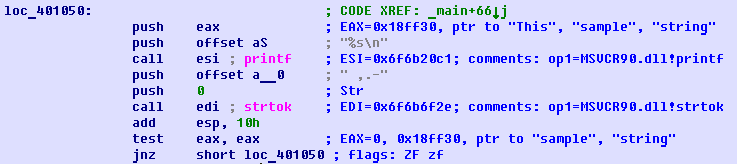
\includegraphics[scale=0.66]{trace_test1.png}
\caption{trace\_test1.png}
\end{figure}

\IFRU{Замечание: "a" это слишком короткая строка для автоматического детектора строк в tracer, поэтому её здесь нет, вместо нее адрес этой строки.}{Note: "a" is too short string for automatic string detector in tracer, that is why it is absent and its address here instead.}

\subsection{\IFRU{Трассируем quicksort()}{Let's trace quicksort()}}

\IFRU{Возьмем известный пример:}{Use well-known example:}

\begin{lstlisting}
//http://cplus.about.com/od/learningc/ss/pointers2_8.htm

/* ex3 Sorting ints with qsort */
//

#include <stdio.h>
#include <stdlib.h>

int comp(const int * a,const int * b) 
{
  if (*a==*b)
    return 0;
  else
    if (*a < *b)
        return -1;
     else
      return 1;
}

int main(int argc, char* argv[])
{
   int numbers[10]={1892,45,200,-98,4087,5,-12345,1087,88,-100000};
   int i;

  /* Sort the array */
  qsort(numbers,10,sizeof(int),comp);
  for (i=0;i<9;i++)
    printf("Number = %d\n",numbers[ i ]);
  return 0;
}
\end{lstlisting}

\IFRU{Трассируем функцию comp():}{Let's trace comp() function:}

\begin{lstlisting}
tracer.exe -l:trace_test2.exe bpf=0x00401030,trace:cc
\end{lstlisting}

\IFRU{Получим после исполнения скрипта в IDA:}{We will get after .idc script execution in IDA:}

\begin{figure}[ht!]
\centering
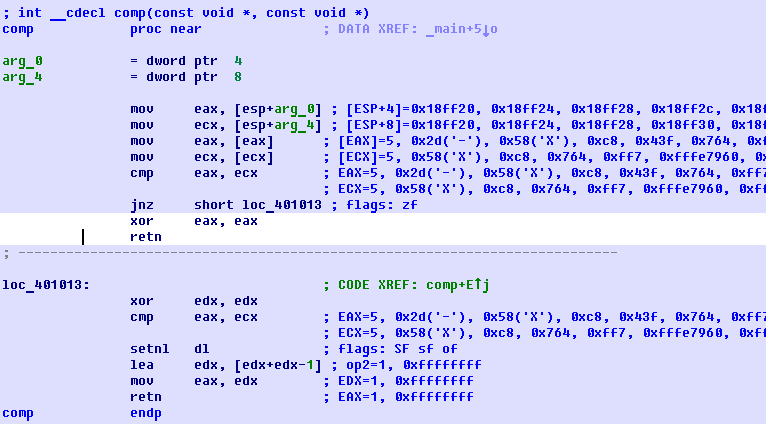
\includegraphics[scale=0.66]{trace_test2.png}
\caption{trace\_test2.png}
\end{figure}

\IFRU{В примере все значения уникальны, одинаковых нет. Таким образом, нет ситуации когда comp() возвращает ноль. Поэтому здесь мы видим что часть comp() возвращающая ноль (xor eax,eax / retn) не была исполнена ни разу.}{In this example all values are unique, there are no equal ones. Therefore, there are no situation when comp() function returning zero. That is why we see that the comp() part returning zero (xor eax,eax / retn) was not executed.}



